\en

\section{Tool architecture}
\label{subsec:architecture}

The Setup step is composed of two components, the Function Breaker and the Code Duplication Finder. the pipeline of this step work as
follow: the Function Parser receives the codebase we are interested, extract the functions of the codebase along with metadata and
creates a new temporary codebase where it function becomes a new code file. The Code Duplication Finder iterate over every pair of 
files in the temporary codebase computing the code duplications and save them in the Code Duplication Database, which is a text file
that stores every code duplication as a triple <function1,function2,similarity>, where function1 and function2 are the functions that 
are a duplication of each other, and similarity is the metric given by the code duplication method utilized, which in our case, it is
the cossine similarity explained in \ref{sec:similarity}. Finally, the Query Responder consumes the temporary codebase and the 
Code Duplication Database to extract code duplication related information as per user request. A diagram to ilustrate the pipeline
can be found in the Figure \ref{fig:diagram}. There is a explanation of how each component work below.

\begin{figure}
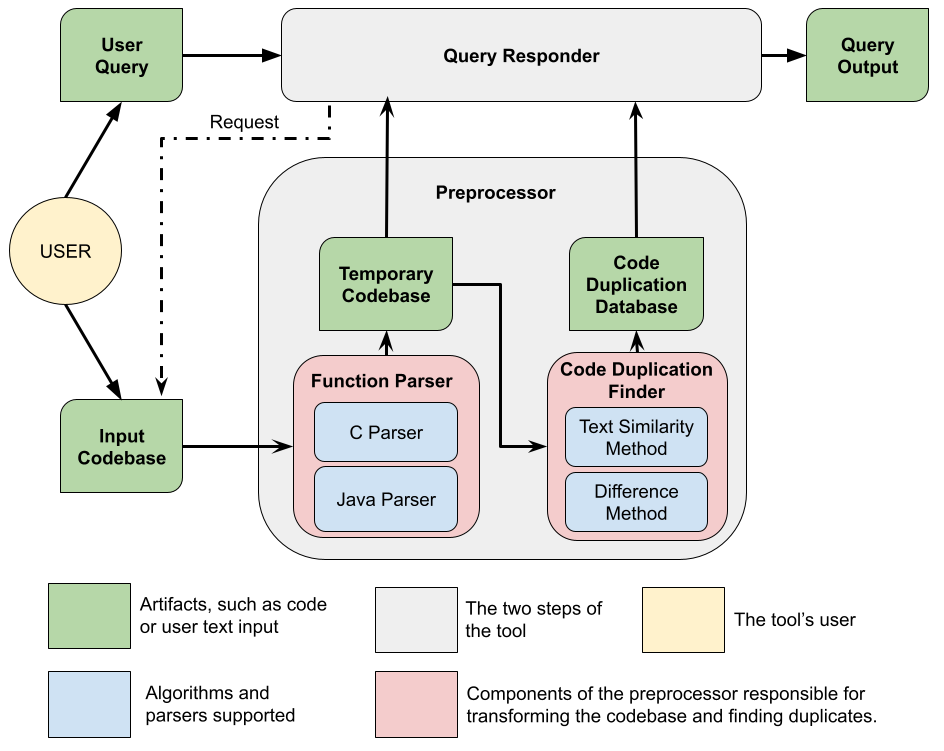
\includegraphics{diagrama_mestrado}
\caption{The architecture diagram demonstrating the relationship between the components.}
\label{fig:diagram}
\end{figure}

\subsection{Input codebase}

The input codebase is expected to be a folder in the machine the tool is running into. All files in the codebase that is not a source
code file from a programming language supported by the tool will be ignored.

\subsection{Function Parser}

The Function Parser receives the input codebase and transforms it into the temporary codebase. The Function Parser iterates through
every source code file from the programming language it support and use a specific programming languague's function 
extractor to extract
every function in the file, for each function extracted we create two new source code files and a metadata file in the temporary codebase
which is represented by the pair \textbf{<source code file, function extracted>}, which represents the source code file the 
function is extracted from and the 
proper function. The first new source code file contains the function's body from the function it represents, while the other
new source code file contains the function's signature, the metadata file 
contains extra relevant information such as function name, the line the function signature starts in the original souce code 
file and the line the function's body ends in the original source code file. The programming language we support at the moment 
is C and Java. Can be found a example of a transform of a source code in the Figure (CREATE APENDIX AND ADD HERE).

About the programming languague's function extractor, we approached this problem in a way that any person comfortable with a language
can adapt our approach to their specific programming language. Usually, the code blocks can be easily extracted from 
source code files, independently if the code blocks are defined by curly brackets or by indentation, and it is possible to
infer if it represents a function's body given how deeply it is in the code context and a few lines before the start 
of the code block. We followed exactly this approach to implement the function extractor for the languagues we implemented. 
As a alternative approach, we can build the syntax tree \citep{compiler} of the programming language and use it to 
extract the functions, which is a more complex task then our main approach. For the programming languages we support, we implemented
it as follow:

\begin{itemize}
	\begin{item}
		\textbf{C}: Given a source code file, we extract every code block from it, maintaining the depth of the code block in
		the code context and som lines of code before the definition of the code block. By the C programming language's grammar, 
		the functions are defined in a global context, with depth of 0. There are other elements with the same depth as functions,
		we differentiate them by analysing if the first non-empty character before the curly brackets of the code block is a close 
		parenthesis, since functions are the only elements that respect this pattern in the C programming language.
	\end{item}
	\begin{item}
		\textbf{Java}: Given a source code file, we extract every code block from it, maintaining the depth of the code block in
		the code context and som lines of code before the definition of the code block. By the Java's grammar, 
		the functions are defined inside classes. There are different depths which we can have functions, as Java accepts inner
		classes. We differentiate functions of other elements by analysing if the first non-empty character before the curly brackets of the code block is a close 
		parenthesis, since there are others elements which also respect this pattern such as for loop, we would need to apply other 
		filters. We chose to only analyse functions of depth 1, which ignores every others elements that respect the previously
		filters, but as counterpart, functions declared inside Inner Classes are not supported by our extractor. We made this choice
		as there are not inner classes on the codebases explored in this work.

	\end{item}
\end{itemize}

\subsection{Temporary codebase}

The temporary codebase is a transformation of the input codebase done by the Function Parser, every function in the input codebase
is represented in the temporary codebase as three files. There are description of each file below and an example of each can found
in the figure (CREATE FIGURE AND ADD HERE).

\begin{itemize}
	\begin{item}
		\textbf{Header file}: This file contains the signature of the function it represents;
	\end{item}
	\begin{item}
		\textbf{Source file:} This file contains the body of the function it represents;
	\end{item}
	\begin{item}
		\textbf{Info file:} This file contains metadata of the function. The information this file contains is:
		the function name, the file name that has the function, the relative path of the file related to the input codebase, 
		the line that the function's signatures starts, the line that the functions body starts, the line that the function's body 
		ends and if there is a line break between the end of the function's signature and the start of the function's body.
		
	\end{item}
\end{itemize}

\subsection{Code Duplication Finder}

The Code Duplication Finder iterates through every pair of source code files in the temporary codebase, which in this context represents
functions of the input codebase, and for every pair of files, we execute a code duplication detection method that computes a metric
that measures of how similar the pair of files are, which we call similarity. Finally, if the similarity is greater of equal then the
minimum similarity threshold (a parameter passed by the user when it executes the Setup step), we store this pair of files along with
it similarity in the Code Duplication Database.

For the code duplication detection method, we visualize the source code files as texts and execute the TF-IDF vector embedding method
implemented by the Gensim library \citep{gensim} and compute the cosine similarity as the similarity metric. We chose this method 
given the alegated Gensim statements about itself performance, being a programming language independent method and the nonnecessity of 
compilable code, which is expected to happen in the temporary codebase as it not stores complete code artifacts. Platis implemented
this code cuplication detection method and distributed it to the public with a MIT license \citep{platistool} \citep{mitlicense}, 
we utilize his implementation as it has some nice to have components such as removing code comments, we do the appropriated changes
in the input and output of his implementation to respect the expected format of our tool. 
It is feasible to change the duplication detection method in a manner similar to what we did with Platis's implementation.

\subsection{Code Duplication Database}

The Code Duplication Database is a text file that contains the duplicated pairs of functions found by the Code Duplication Finder, 
the first line of the file contains a number that represents the number of the duplicated pairs, after that, there is 
a line of each duplicated pairs that contains the path of the functions in the temporary codebase and the similarity metric of the 
pair. A example of the Code Duplication Database can be found in the figure (ADD FIGURE HERE). 

\subsection{Setup step}

\label{subsec:setup}

The Setup step is a procedure executed by the user once per codebase. The Setup step receives the input codebase and the minimum
similarity metric value to a pair of functions to be considered a duplication, then it executes the Function Parser and the Code 
Duplication Finder, to generate the temporary codebase and the Code Duplication Database, which will be later used by the Query
Responder step. The value of the minimum similarity metric is to reduce the Code Duplication Database, which optimize the
memory usage and the computational cost of the Query Responder step. For example, if this parameter does not exist and we work in 
a codebase of $10000$ functions and supposing each relative path plus the function name have $50$ charactes, the Code Duplication 
Database will be a file of size approximately $5000^2 \times 50 ~= 5$ Gigabytes, as it is not expected to a real large codebase 
to the majority of pairs of functions be a duplication of each other, this number can be reduced dramastically.

\subsection{Query Responder step}

The Query Responder step is the component that the user executes multiples times to consult information about code duplication in
a codebase that was previously preprocessed by the Setup step. The Query Responder step consumes the temporary codebase and the 
Code Duplication Database created by the Setup step. This component implements all the tool's functionalities exposed 
for the user, which are described in the \ref{subsec:func}.

